
%% bare_jrnl.tex
%% V1.4b
%% 2015/08/26
%% by Michael Shell
%% see http://www.michaelshell.org/
%% for current contact information.
%%
%% This is a skeleton file demonstrating the use of IEEEtran.cls
%% (requires IEEEtran.cls version 1.8b or later) with an IEEE
%% journal paper.
%%
%% Support sites:
%% http://www.michaelshell.org/tex/ieeetran/
%% http://www.ctan.org/pkg/ieeetran
%% and
%% http://www.ieee.org/

%%*************************************************************************
%% Legal Notice:
%% This code is offered as-is without any warranty either expressed or
%% implied; without even the implied warranty of MERCHANTABILITY or
%% FITNESS FOR A PARTICULAR PURPOSE! 
%% User assumes all risk.
%% In no event shall the IEEE or any contributor to this code be liable for
%% any damages or losses, including, but not limited to, incidental,
%% consequential, or any other damages, resulting from the use or misuse
%% of any information contained here.
%%
%% All comments are the opinions of their respective authors and are not
%% necessarily endorsed by the IEEE.
%%
%% This work is distributed under the LaTeX Project Public License (LPPL)
%% ( http://www.latex-project.org/ ) version 1.3, and may be freely used,
%% distributed and modified. A copy of the LPPL, version 1.3, is included
%% in the base LaTeX documentation of all distributions of LaTeX released
%% 2003/12/01 or later.
%% Retain all contribution notices and credits.
%% ** Modified files should be clearly indicated as such, including  **
%% ** renaming them and changing author support contact information. **
%%*************************************************************************


% *** Authors should verify (and, if needed, correct) their LaTeX system  ***
% *** with the testflow diagnostic prior to trusting their LaTeX platform ***
% *** with production work. The IEEE's font choices and paper sizes can   ***
% *** trigger bugs that do not appear when using other class files.       ***                          ***
% The testflow support page is at:
% http://www.michaelshell.org/tex/testflow/



\documentclass[journal]{IEEEtran}
%
% If IEEEtran.cls has not been installed into the LaTeX system files,
% manually specify the path to it like:
% \documentclass[journal]{../sty/IEEEtran}





% Some very useful LaTeX packages include:
% (uncomment the ones you want to load)


% *** MISC UTILITY PACKAGES ***
%
\usepackage{ifpdf}
% Heiko Oberdiek's ifpdf.sty is very useful if you need conditional
% compilation based on whether the output is pdf or dvi.
% usage:
 \ifpdf
   % pdf code
 \else
   % dvi code
 \fi
% The latest version of ifpdf.sty can be obtained from:
% http://www.ctan.org/pkg/ifpdf
% Also, note that IEEEtran.cls V1.7 and later provides a builtin
% \ifCLASSINFOpdf conditional that works the same way.
% When switching from latex to pdflatex and vice-versa, the compiler may
% have to be run twice to clear warning/error messages.






% *** CITATION PACKAGES ***
%
\usepackage{cite}
% cite.sty was written by Donald Arseneau
% V1.6 and later of IEEEtran pre-defines the format of the cite.sty package
% \cite{} output to follow that of the IEEE. Loading the cite package will
% result in citation numbers being automatically sorted and properly
% "compressed/ranged". e.g., [1], [9], [2], [7], [5], [6] without using
% cite.sty will become [1], [2], [5]--[7], [9] using cite.sty. cite.sty's
% \cite will automatically add leading space, if needed. Use cite.sty's
% noadjust option (cite.sty V3.8 and later) if you want to turn this off
% such as if a citation ever needs to be enclosed in parenthesis.
% cite.sty is already installed on most LaTeX systems. Be sure and use
% version 5.0 (2009-03-20) and later if using hyperref.sty.
% The latest version can be obtained at:
% http://www.ctan.org/pkg/cite
% The documentation is contained in the cite.sty file itself.






% *** GRAPHICS RELATED PACKAGES ***
%
\ifCLASSINFOpdf
 \usepackage[pdftex]{graphicx}
% declare the path(s) where your graphic files are
% \graphicspath{{../pdf/}{../jpeg/}}
% and their extensions so you won't have to specify these with
% every instance of \includegraphics
 \DeclareGraphicsExtensions{.pdf,.jpeg,.png}
\else
% or other class option (dvipsone, dvipdf, if not using dvips). graphicx
% will default to the driver specified in the system graphics.cfg if no
% driver is specified.
 \usepackage[dvips]{graphicx}
% declare the path(s) where your graphic files are
% \graphicspath{{../eps/}}
% and their extensions so you won't have to specify these with
% every instance of \includegraphics
 \DeclareGraphicsExtensions{.eps}
\fi
% graphicx was written by David Carlisle and Sebastian Rahtz. It is
% required if you want graphics, photos, etc. graphicx.sty is already
% installed on most LaTeX systems. The latest version and documentation
% can be obtained at: 
% http://www.ctan.org/pkg/graphicx
% Another good source of documentation is "Using Imported Graphics in
% LaTeX2e" by Keith Reckdahl which can be found at:
% http://www.ctan.org/pkg/epslatex
%
% latex, and pdflatex in dvi mode, support graphics in encapsulated
% postscript (.eps) format. pdflatex in pdf mode supports graphics
% in .pdf, .jpeg, .png and .mps (metapost) formats. Users should ensure
% that all non-photo figures use a vector format (.eps, .pdf, .mps) and
% not a bitmapped formats (.jpeg, .png). The IEEE frowns on bitmapped formats
% which can result in "jaggedy"/blurry rendering of lines and letters as
% well as large increases in file sizes.
%
% You can find documentation about the pdfTeX application at:
% http://www.tug.org/applications/pdftex





% *** MATH PACKAGES ***
%
\usepackage{amsmath}
% A popular package from the American Mathematical Society that provides
% many useful and powerful commands for dealing with mathematics.
%
% Note that the amsmath package sets \interdisplaylinepenalty to 10000
% thus preventing page breaks from occurring within multiline equations. Use:
%\interdisplaylinepenalty=2500
% after loading amsmath to restore such page breaks as IEEEtran.cls normally
% does. amsmath.sty is already installed on most LaTeX systems. The latest
% version and documentation can be obtained at:
% http://www.ctan.org/pkg/amsmath





% *** SPECIALIZED LIST PACKAGES ***
%
\usepackage{algorithmic}
% algorithmic.sty was written by Peter Williams and Rogerio Brito.
% This package provides an algorithmic environment fo describing algorithms.
% You can use the algorithmic environment in-text or within a figure
% environment to provide for a floating algorithm. Do NOT use the algorithm
% floating environment provided by algorithm.sty (by the same authors) or
% algorithm2e.sty (by Christophe Fiorio) as the IEEE does not use dedicated
% algorithm float types and packages that provide these will not provide
% correct IEEE style captions. The latest version and documentation of
% algorithmic.sty can be obtained at:
% http://www.ctan.org/pkg/algorithms
% Also of interest may be the (relatively newer and more customizable)
% algorithmicx.sty package by Szasz Janos:
% http://www.ctan.org/pkg/algorithmicx




% *** ALIGNMENT PACKAGES ***
%
\usepackage{array}
% Frank Mittelbach's and David Carlisle's array.sty patches and improves
% the standard LaTeX2e array and tabular environments to provide better
% appearance and additional user controls. As the default LaTeX2e table
% generation code is lacking to the point of almost being broken with
% respect to the quality of the end results, all users are strongly
% advised to use an enhanced (at the very least that provided by array.sty)
% set of table tools. array.sty is already installed on most systems. The
% latest version and documentation can be obtained at:
% http://www.ctan.org/pkg/array


% IEEEtran contains the IEEEeqnarray family of commands that can be used to
% generate multiline equations as well as matrices, tables, etc., of high
% quality.




% *** SUBFIGURE PACKAGES ***
%\ifCLASSOPTIONcompsoc
%  \usepackage[caption=false,font=normalsize,labelfont=sf,textfont=sf]{subfig}
%\else
%  \usepackage[caption=false,font=footnotesize]{subfig}
%\fi
% subfig.sty, written by Steven Douglas Cochran, is the modern replacement
% for subfigure.sty, the latter of which is no longer maintained and is
% incompatible with some LaTeX packages including fixltx2e. However,
% subfig.sty requires and automatically loads Axel Sommerfeldt's caption.sty
% which will override IEEEtran.cls' handling of captions and this will result
% in non-IEEE style figure/table captions. To prevent this problem, be sure
% and invoke subfig.sty's "caption=false" package option (available since
% subfig.sty version 1.3, 2005/06/28) as this is will preserve IEEEtran.cls
% handling of captions.
% Note that the Computer Society format requires a larger sans serif font
% than the serif footnote size font used in traditional IEEE formatting
% and thus the need to invoke different subfig.sty package options depending
% on whether compsoc mode has been enabled.
%
% The latest version and documentation of subfig.sty can be obtained at:
% http://www.ctan.org/pkg/subfig




% *** FLOAT PACKAGES ***
%
%\usepackage{fixltx2e}
% fixltx2e, the successor to the earlier fix2col.sty, was written by
% Frank Mittelbach and David Carlisle. This package corrects a few problems
% in the LaTeX2e kernel, the most notable of which is that in current
% LaTeX2e releases, the ordering of single and double column floats is not
% guaranteed to be preserved. Thus, an unpatched LaTeX2e can allow a
% single column figure to be placed prior to an earlier double column
% figure.
% Be aware that LaTeX2e kernels dated 2015 and later have fixltx2e.sty's
% corrections already built into the system in which case a warning will
% be issued if an attempt is made to load fixltx2e.sty as it is no longer
% needed.
% The latest version and documentation can be found at:
% http://www.ctan.org/pkg/fixltx2e


%\usepackage{stfloats}
% stfloats.sty was written by Sigitas Tolusis. This package gives LaTeX2e
% the ability to do double column floats at the bottom of the page as well
% as the top. (e.g., "\begin{figure*}[!b]" is not normally possible in
% LaTeX2e). It also provides a command:
%\fnbelowfloat
% to enable the placement of footnotes below bottom floats (the standard
% LaTeX2e kernel puts them above bottom floats). This is an invasive package
% which rewrites many portions of the LaTeX2e float routines. It may not work
% with other packages that modify the LaTeX2e float routines. The latest
% version and documentation can be obtained at:
% http://www.ctan.org/pkg/stfloats
% Do not use the stfloats baselinefloat ability as the IEEE does not allow
% \baselineskip to stretch. Authors submitting work to the IEEE should note
% that the IEEE rarely uses double column equations and that authors should try
% to avoid such use. Do not be tempted to use the cuted.sty or midfloat.sty
% packages (also by Sigitas Tolusis) as the IEEE does not format its papers in
% such ways.
% Do not attempt to use stfloats with fixltx2e as they are incompatible.
% Instead, use Morten Hogholm'a dblfloatfix which combines the features
% of both fixltx2e and stfloats:
%
%\usepackage{dblfloatfix}
% The latest version can be found at:
% http://www.ctan.org/pkg/dblfloatfix




%\ifCLASSOPTIONcaptionsoff
%  \usepackage[nomarkers]{endfloat}
% \let\MYoriglatexcaption\caption
% \renewcommand{\caption}[2][\relax]{\MYoriglatexcaption[#2]{#2}}
%\fi
% endfloat.sty was written by James Darrell McCauley, Jeff Goldberg and 
% Axel Sommerfeldt. This package may be useful when used in conjunction with 
% IEEEtran.cls'  captionsoff option. Some IEEE journals/societies require that
% submissions have lists of figures/tables at the end of the paper and that
% figures/tables without any captions are placed on a page by themselves at
% the end of the document. If needed, the draftcls IEEEtran class option or
% \CLASSINPUTbaselinestretch interface can be used to increase the line
% spacing as well. Be sure and use the nomarkers option of endfloat to
% prevent endfloat from "marking" where the figures would have been placed
% in the text. The two hack lines of code above are a slight modification of
% that suggested by in the endfloat docs (section 8.4.1) to ensure that
% the full captions always appear in the list of figures/tables - even if
% the user used the short optional argument of \caption[]{}.
% IEEE papers do not typically make use of \caption[]'s optional argument,
% so this should not be an issue. A similar trick can be used to disable
% captions of packages such as subfig.sty that lack options to turn off
% the subcaptions:
% For subfig.sty:
% \let\MYorigsubfloat\subfloat
% \renewcommand{\subfloat}[2][\relax]{\MYorigsubfloat[]{#2}}
% However, the above trick will not work if both optional arguments of
% the \subfloat command are used. Furthermore, there needs to be a
% description of each subfigure *somewhere* and endfloat does not add
% subfigure captions to its list of figures. Thus, the best approach is to
% avoid the use of subfigure captions (many IEEE journals avoid them anyway)
% and instead reference/explain all the subfigures within the main caption.
% The latest version of endfloat.sty and its documentation can obtained at:
% http://www.ctan.org/pkg/endfloat
%
% The IEEEtran \ifCLASSOPTIONcaptionsoff conditional can also be used
% later in the document, say, to conditionally put the References on a 
% page by themselves.




% *** PDF, URL AND HYPERLINK PACKAGES ***
%
\usepackage{url}
% url.sty was written by Donald Arseneau. It provides better support for
% handling and breaking URLs. url.sty is already installed on most LaTeX
% systems. The latest version and documentation can be obtained at:
% http://www.ctan.org/pkg/url
% Basically, \url{my_url_here}.




% *** Do not adjust lengths that control margins, column widths, etc. ***
% *** Do not use packages that alter fonts (such as pslatex).         ***
% There should be no need to do such things with IEEEtran.cls V1.6 and later.
% (Unless specifically asked to do so by the journal or conference you plan
% to submit to, of course. )


% correct bad hyphenation here
\hyphenation{op-tical net-works semi-conduc-tor fre-quency}


\usepackage[utf8]{inputenc}
\usepackage[english]{babel}

\begin{document}
	%
	% paper title
	% Titles are generally capitalized except for words such as a, an, and, as,
	% at, but, by, for, in, nor, of, on, or, the, to and up, which are usually
	% not capitalized unless they are the first or last word of the title.
	% Linebreaks \\ can be used within to get better formatting as desired.
	% Do not put math or special symbols in the title.
	\title{Customer Behavioural Analytic\\ on Food Delivery Services}
	%
	%
	% author names and IEEE memberships
	% note positions of commas and nonbreaking spaces ( ~ ) LaTeX will not break
	% a structure at a ~ so this keeps an author's name from being broken across
	% two lines.
	% use \thanks{} to gain access to the first footnote area
	% a separate \thanks must be used for each paragraph as LaTeX2e's \thanks
	% was not built to handle multiple paragraphs
	%
	
	\author{Lee~Kang~Wenn,
		Chan~Peck~Hui
		and Yang~Poh~Yee}% <-this % stops a space
%		\thanks{M. Shell was with the Department
%			of Electrical and Computer Engineering, Georgia Institute of Technology, Atlanta,
%			GA, 30332 USA e-mail: (see http://www.michaelshell.org/contact.html).}% <-this % stops a space
%		\thanks{J. Doe and J. Doe are with Anonymous University.}% <-this % stops a space
%		\thanks{Manuscript received April 19, 2005; revised August 26, 2015.}}
	
	% note the % following the last \IEEEmembership and also \thanks - 
	% these prevent an unwanted space from occurring between the last author name
	% and the end of the author line. i.e., if you had this:
	% 
	% \author{....lastname \thanks{...} \thanks{...} }
	%                     ^------------^------------^----Do not want these spaces!
	%
	% a space would be appended to the last name and could cause every name on that
	% line to be shifted left slightly. This is one of those "LaTeX things". For
	% instance, "\textbf{A} \textbf{B}" will typeset as "A B" not "AB". To get
	% "AB" then you have to do: "\textbf{A}\textbf{B}"
	% \thanks is no different in this regard, so shield the last } of each \thanks
	% that ends a line with a % and do not let a space in before the next \thanks.
	% Spaces after \IEEEmembership other than the last one are OK (and needed) as
	% you are supposed to have spaces between the names. For what it is worth,
	% this is a minor point as most people would not even notice if the said evil
	% space somehow managed to creep in.
	
	
	
	% The paper headers
	\markboth{Innovate Malaysia Design Competition 2018}%
	{Shell \MakeLowercase{\textit{et al.}}: Bare Demo of IEEEtran.cls for IEEE Journals}
	% The only time the second header will appear is for the odd numbered pages
	% after the title page when using the twoside option.
	% 
	% *** Note that you probably will NOT want to include the author's ***
	% *** name in the headers of peer review papers.                   ***
	% You can use \ifCLASSOPTIONpeerreview for conditional compilation here if
	% you desire.
	
	
	
	
	% If you want to put a publisher's ID mark on the page you can do it like
	% this:
	%\IEEEpubid{0000--0000/00\$00.00~\copyright~2015 IEEE}
	% Remember, if you use this you must call \IEEEpubidadjcol in the second
	% column for its text to clear the IEEEpubid mark.
	
	
	
	% use for special paper notices
	%\IEEEspecialpapernotice{(Invited Paper)}
	
	
	
	
	% make the title area
	\maketitle
	
	% As a general rule, do not put math, special symbols or citations
	% in the abstract or keywords.
	\begin{abstract}
		As penetration of smart phones and mobile applications increases, the technology is going to trigger a massive influx of big data. Consumer analytic is at the epicentre of a big data revolution. Technology helps capture rich and plentiful data on consumer behaviour in real time. Therefore, this project aims to use machine learning to build a more efficient and simpler consumer analytic model for small and medium-sized enterprise that does not have much resources to carry out data analysis.
	\end{abstract}
	
	% Note that keywords are not normally used for peerreview papers.
	\begin{IEEEkeywords}
		Churn Analysis, Customer behavioural Analysis, Data mining, Decision trees, K-means clustering, Market Segmentation, Neural networks, RFM
	\end{IEEEkeywords}
	
	
	
	
	
	
	% For peer review papers, you can put extra information on the cover
	% page as needed:
	% \ifCLASSOPTIONpeerreview
	% \begin{center} \bfseries EDICS Category: 3-BBND \end{center}
	% \fi
	%
	% For peerreview papers, this IEEEtran command inserts a page break and
	% creates the second title. It will be ignored for other modes.
	\IEEEpeerreviewmaketitle
	
	
	
	\section{Introduction}
	% The very first letter is a 2 line initial drop letter followed
	% by the rest of the first word in caps.
	% 
	% form to use if the first word consists of a single letter:
	% \IEEEPARstart{A}{demo} file is ....
	% 
	% form to use if you need the single drop letter followed by
	% normal text (unknown if ever used by the IEEE):
	% \IEEEPARstart{A}{}demo file is ....
	% 
	% Some journals put the first two words in caps:
	% \IEEEPARstart{T}{his demo} file is ....
	% 
	% Here we have the typical use of a "T" for an initial drop letter
	% and "HIS" in caps to complete the first word.
	\IEEEPARstart{T}{he} massive increase in the amount of data collected and stored by organizations around the world over the past few decades is evident. In conjunction with this, the ability to access and analyse this data is quickly becoming more and more important. However, some firms do not have the resources to perform consumer analytic and it’s often inaccurate \cite{Erevelles2016-oa}. Analysing consumer data often requires huge amount of time, manpower, and professionals, which leads to high cost for small organization to carry out data analysis.
	
	This project aims to achieve several objectives. The main objective of this project is to extract semantic customers behavioural information through data collected from a food delivery company, Running Man. Customer behavioural refers to actions done by customers on the website and number of customers visiting the website. 
	
	The data is then processed by going through features extraction, pre-processing and input into machine learning algorithm for output. We will also explore the most accurate prediction model for the project. We will then provide suggestions such as cross-selling products, peak hour prediction and conducting promotions events based on the output from the prediction model.
	
	Data extracted that are trained by machine learning will be examined in terms of predictive accuracy in order to be applied in real-life situation. By examining information such as customers’ purchasing behaviour, such information can help the management to make better decision in terms of marketing and planning, hence increases sales performance \cite{Raorane2011-xu}.

	Investigating customer behaviour in retail contexts is essential to obtain various formal indicators that are interesting from the marketing research viewpoint such as the conversion rates, to further improve the food delivery experiences. Being able to analyse and predict market and customer behaviour with big data is a new paradigm shift for small and medium-sized enterprises (SMEs). When it is implemented correctly, it can yield increased flexibility, productivity responsiveness, anticipation and ability to meet customer need through capturing blind spots and making better decisions \cite{Sen2016-mw}.
		
	\section{Literature review}
	More and more companies embrace Artificial Intelligence to assist them in decision making. For example, Ford Motors is using consumer analytic to start its own revolution in product innovation and design\cite{Erevelles2016-oa}. Ford facilitates product innovation in a rapid manner using Big Data without waiting for insights from traditional research such as focus groups and surveys \cite{Satell2014-mg}.
	
	This solution benefits two parties: the consumer and the merchant. The system can be implemented to provide “personalized shopping experience or services to the consumer”. Furthermore, the system can also be implemented to provide sophisticated insights to assist top management in decision making, product perfecting, and more importantly, customer satisfaction. When a firm embraces new technology and constantly seeks for transformation of knowledge, the knowledge creation process grows exponentially. With these resources, a firm can improve performance better than without resources, thus the resources are considered valuable \cite{Kozlenkova2014-yc}.
	
	Before a consumer prediction analytic model is created, an iteration of process is needed.
	
	\begin{figure}[!ht]
		\centering
		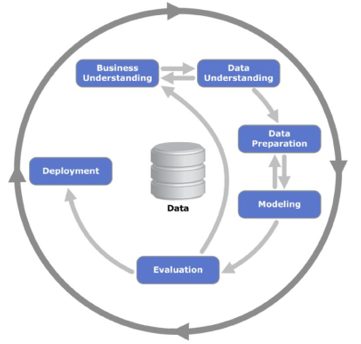
\includegraphics[scale=0.5]{process}
		\caption{Process of modelling consumer prediction analytic.}
	\end{figure}

The first step is business understanding. We need to analyse and understand the business logic and the policy of the business in business perspective. Next up is data understanding. We need to study all the available data and investigate the relationship between all available data in order to perform data mining correctly. Data preparation is then carried out to perform ensure all the data is valid for the modelling. In modelling, various techniques are applied into the model and tested. The most suitable technique is then proceed to evaluation. In evaluation, the model is evaluated in different measures such as accuracy, performance and efficiency. Over-fitting of model might occur therefore an evaluation of the model is needed to make sure the model can be then be deployed. Lastly, the model will be deployed into real system to start servicing the user.

\section{Consumer Behavioural Analytic}
Consumer Behavioural Analytic is the analysis of the past data on what the customers do and how they act in a manner that will reflect in what they do and how they will react in the future. Consumer analytic is important to a company, it brings benefits such as understanding customers’ need, customers’ purchasing power and many more \cite{Erevelles2016-oa}. If there is a strong behavioural analytic exists, it can be widely used in helping to build a smarter businesses with social commerce so that retailers can now record and track the customers on how do they buy, what are their choice criteria, when and how frequent do they buy and their oath channels when checking out products.

\begin{figure}[!ht]
	\centering
	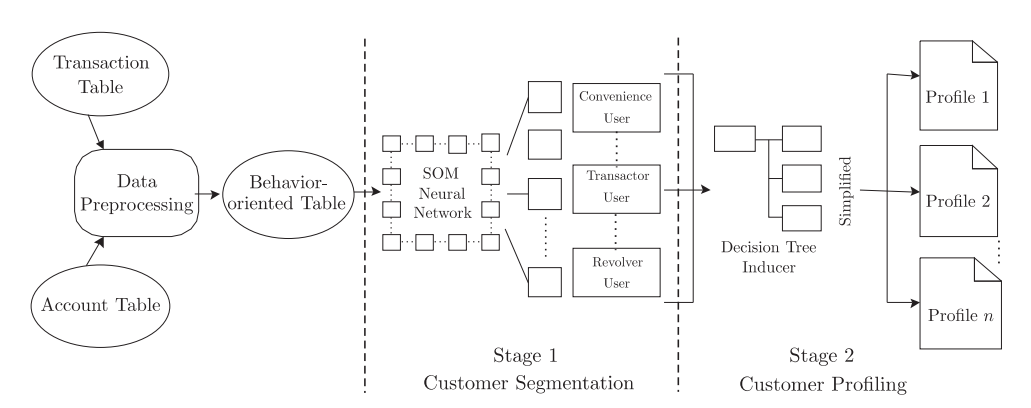
\includegraphics[scale=0.2]{framework}
	\caption{The two-stage framework of consumer behaviour analysis\cite{Hsieh2009-rc}.}
\end{figure}

The study of consumer analytic lies at the junction of Big Data and consumer behaviour. Big data is a hot issue in today’s world. 4.4 Zettabytes of data exist in the digital universe today, by 2020, the digital universe is expected to reach 44 zettabytes \cite{Idc2014-ey}. Since data provide behavioural insights about consumers; marketers are able to translate those insights into market advantage. Big data is a top business priority and drives enormous opportunity for business improvement \cite{Kennedy2011-dt}. Nevertheless, the first problem is that manually analyses the conglomeration of raw data to gain insights is inefficient and ineffective.

Consumer analytic can be performed by deductive or inductive approaches, where deductive approaches interpret consumer behaviour based on existing theories and model, while inductive approaches do not make any assumptions or hypothesis before the interpretation. Deductive approaches have been widely used, providing good results. However, the need to obtain even more insights has directed marketers’ interest towards inductive prediction approaches. Studies have shown that using inductive approaches consumer analytic can advance the understanding of marketing phenomena more compared to using deductive approaches \cite{Erevelles2016-oa}. Without interconnecting the relationship among consumers’ purchases, customers’ flow and path on the web, deductive approaches would be inaccurate.

\section{Supervised and Unsupervised Machine Learning Algorithm}
\subsection{Ordinary Least Square}
In statistical modelling, regression analysis is a statistical process which estimates the relationship among variables and the outcome of output for this statistical model is continuous real value, also known as function approximation \cite{Pedregosa2011-ac}. There are many regression model that exists, such as Ridge Regression (impose penalty on size of coefficient), Lasso Regression (estimates sparse coefficients).

Ordinary Least Squares, also known as Linear Regression, is one of the simplest regression model in regression models. Linear Regression fits data with the best hyper-plane which “goes through” the points. For each point the differences between the predicted point and the actual observation is the residue.

\begin{figure}[!ht]
	\centering
	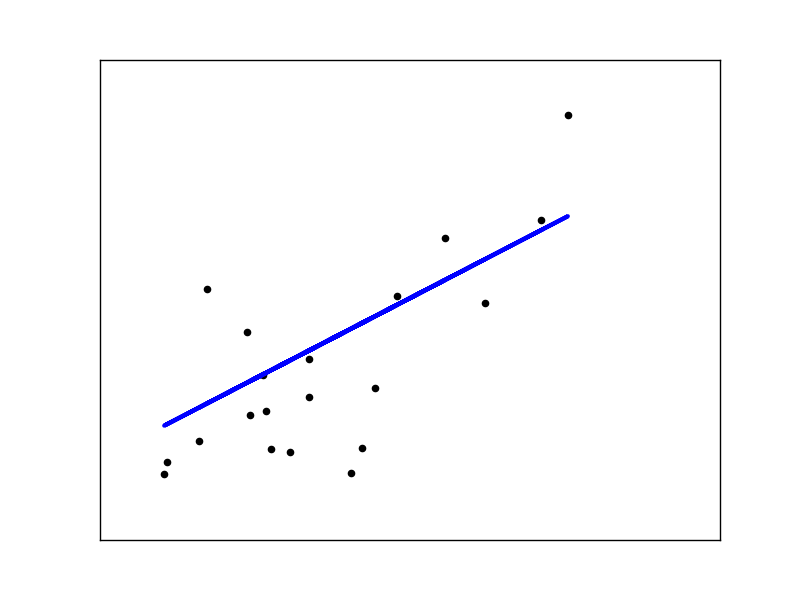
\includegraphics[scale=0.2]{linear}
	\caption{A linear regression visualization.}
\end{figure}

Linear regression is an approach to find out the sum of error in the dataset. Gradient descent is an iterative method to find the minimum of a function. Gradient descent can also be replaced by gradient ascent to determine the maximum of a function.

Gradient descent starts with an initial set of data; in each step, it decreases each data in proportion to its partial derivative. There will a be gradient descent step size, also known as learning rate, along with features and the data is given as input to the learning algorithm. The partial derivative specifies how much a small change in the data would change the error. 

Consider minimizing the sum-of-squares error. The error is a sum over the examples. The partial derivative of a sum is the sum of the partial derivatives. Thus, we can consider each example separately and consider how much it changes the data.

Linear regression computes the least squares solution using a singular value decomposition of X. If X is a matrix of size (n, p) this method has a cost of $O\left(n{p}^{2}\right)$, assuming that $n\ge p$. If the data used for regression is gigantic, the machine will need longer time to process all the data. 

However, Linear regression only limited to linear relationship, which means it only looks at dependent and independent variables. Some of the data might not have straight relationship between two of the variables. Also, linear regression is sensitive to outliers. Outliers will affect the linear relationship plotted thus affect the accuracy of the relationship \cite{Sciencing2017-qw}.

Linear Regression is a very powerful statistical technique and can be used to generate insight on the data that we, human usually could not understand without plotting the graph. For example, linear regression can be used in business sector to generate insight on consumer behavior, understanding business and factors influencing profitability. By conducting a linear analysis on the sales data of the company, the company could forecast their sales in the future \cite{Xu2016-hp}.

\subsection{Support Vector Machine}
Support vector machines (SVMs) are a set of supervised learning methods used for classification, regression and outliers detection. It is mostly used in classification problems. In SVM, each data item is plotted as a point in n-dimensional space, where n is the number of features in the dataset) with the value of each feature being the value of a particular coordinate. Then, classification will be performed by finding the hyperplane that differentiate the two classes very well \cite{Ray2017-ty}.

\begin{figure}[!ht]
	\centering
	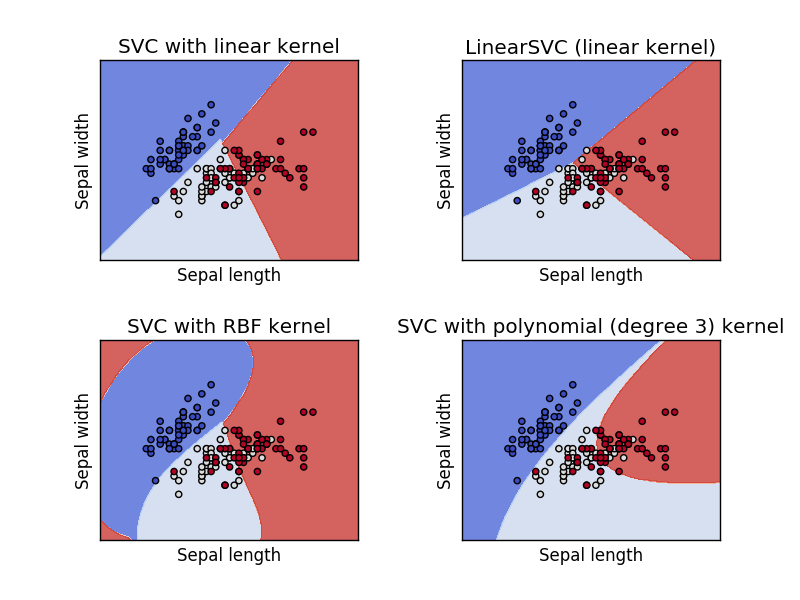
\includegraphics[scale=0.3]{svc}
	\caption{Support Vector Machine visualization.}
\end{figure}

Support Vectors are simply the coordinates of individual observation. Support Vector Machine is a frontier which best segregates the two classes (hyperplane/line).
SVM can identify the right hyperplane by maximizing the distances (margin) between nearest data point (either class).

SVM also has a feature to ignore outliers and find the hyperplane that has maximum margin. Hence, we can say, SVM is robust to outliers.

SVM can also solve problem where the dataset could not have linear hyperplane between the classes. It solves this problem by introducing an additional feature. The machine replot the plane based on the new feature - equation on axis x and z, for example.

\subsection{Random Forest}
Decision Trees are a non-parametric supervised learning method used for classification and regression. Decision tree learning is one of the most successful techniques for supervised classification learning. Decision tree model aims to create a model that predicts the value of a target variable by learning simple decision rules inferred from the data features.	

\begin{figure}[!ht]
	\centering
	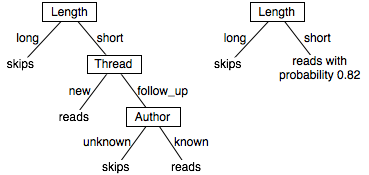
\includegraphics[scale=0.5]{tree}
	\caption{A decision tree visualization.}
\end{figure}

A decision trees, also known as classification tree, is a flowchart like tree structure, which each internal (non-leaf) node is labeled an input feature. The branch (arcs coming from a node) represents an outcome of the test. Each leaf of the tree is labeled with a class name or class distribution. Random forest contain a forest of decision tree \cite{Pedregosa2011-ac}.

Random Forest belongs to a larger class of machine learning algorithms called ensemble methods. Ensemble learning involves the combination of several models to solve a single prediction problem.

\begin{figure}[!ht]
	\centering
	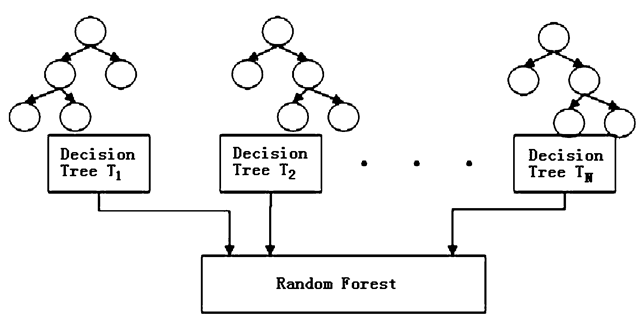
\includegraphics[scale=0.2]{forest}
	\caption{A random forest visualization.}
\end{figure}

In random forests, each tree in the ensemble is built from a sample drawn with replacement (eg. bootstrap sample) from the training set. In addition, when splitting a node during the construction of the tree, the split that is chosen is no longer the best split among all features. Instead, the split that is picked is the best split among a random subset of the features. As a result of this randomness, the bias of the forest usually slightly increases (with respect to the bias of a single non-random tree) but, due to averaging, its variance also decreases, usually more than compensating for the increase in bias, hence yielding an overall better model.

\subsection{Artificial Neural Network}
An Artificial Neural Network (ANN) is an information processing paradigm that is inspired by the way biological nervous systems, such as the brain, process information \cite{Specht1990-nr}. The key element of this paradigm is the novel structure of the information processing system. It is composed of a large number of highly interconnected processing elements (neurons) working in unison to solve specific problems. ANNs, like people, learn by example. An ANN is configured for a specific application, such as pattern recognition or data classification, through a learning process. Learning in biological systems involves adjustments to the synaptic connections that exist between the neurons. This is true of ANNs as well.

\begin{figure}[!ht]
	\centering
	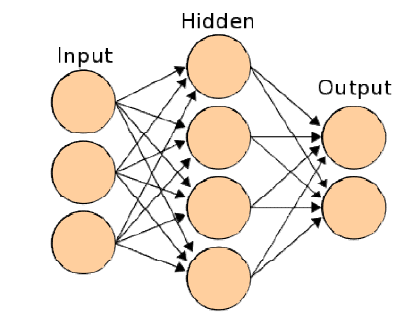
\includegraphics[scale=0.5]{ANN}
	\caption{Artificial Neural Network visualization.}
\end{figure}


The input is the number of input, the data inputted will be push into hidden layer, and the hidden layer will process the information and output the data. In neural network, the input layer, hidden layer and output layer are similar as our human brain, where nerves is nodes in this case.

\subsection{K-means clustering}
K-means \cite{MacQueen1967-ja} is one of the simplest unsupervised learning algorithms that solve the well known clustering problem. The procedure follows a simple and easy way to classify a given data set through a certain number of clusters (assume k clusters) fixed a priori. The main idea is to define k centroids, one for each cluster.

It is typically used for scenarios like understanding the population demographics, market segmentation, social media trends, anomaly detection, etc. where the clusters are unknown to begin with.

\begin{figure}[!ht]
	\centering
	
\includegraphics[scale=0.5]{kmeans}
	\caption{Analytic Process Model visualization.}
\end{figure}

In training phase of K-Means, K observations are arbitrarily selected (known as centroids). Each point in the vector space is assigned to a cluster represented by nearest (euclidean distance) centroid. Once the clusters are formed, for each cluster the centroid is updated to the mean of all cluster members. And the cluster formation restarts with new centroids. This repeats until the centroids themselves become mean of clusters, i.e., when updating centroids to mean doesn’t change them. The prediction of a test observation is done based on nearest centroid.

\section{Research Methodology}
\subsection{Analytic Process Model}
Prediction model is part of analytics process in data science. It is a model which study historical data to forecasting and make prediction for future. The prediction model is using statistics number to show the likelihood of that particular prediction will happen in future. Table 2.3.1 below with diagram and description will describe the whole process from data collection stage until prediction making stage.

\begin{figure}[!ht]
	\centering
	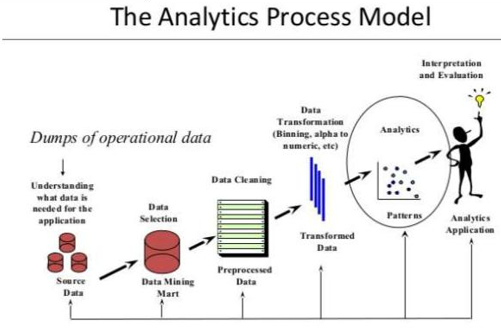
\includegraphics[scale=0.4]{analytics}
	\caption{Analytic Process Model visualization.}
\end{figure}

\begin{table}[!ht]
	\renewcommand{\arraystretch}{1.3}
	\setlength\extrarowheight{2.5pt}
	\caption{The Analytic Process Model and explanation.}
	\label{Analytic Proces Model}
	\centering	
% \usepackage{array} is required
\begin{tabular}{|l|>{\raggedright\arraybackslash}p{5cm}|}
	\hline 
	Process & Explanation \\ 
	\hline 
	Source Data & Unstructured data from various places such as: excel files, log book \\ 
	\hline 
	Data Mining & Retrive the data from source data and discover their correlation and pattern. \\ 
	\hline 
	Preprocess Data & Data filtering process to ensure data is having minimal error before proceed to the next step. For example, deciding what to do with missing data - discard outlier or replace with values. \\ 
	\hline 
	Transform Data & Because data is stored in various form and format, therefore data transformation is needed to transform the data into suitable data format for machine learning. \\ 
	\hline 
	Analytic & Visualizing the information so that it’s easier to understand, in terms of diagrams such as histogram, bar chart. \\ 
	\hline 
	Analytic Application & Extract knowledge from the visualized information and apply the knowledge into application. \\ 
	\hline 
\end{tabular} 
\end{table}

\subsection{The dataset}
The dataset that we managed to collect are the transaction data from a food delivery services. Here are the columns available in the data set.

\begin{table}[!ht]
	\renewcommand{\arraystretch}{1.3}
	\setlength\extrarowheight{2.5pt}
	\caption{Data description}
	\centering
% \usepackage{array} is required
\begin{tabular}{|l|l|>{\raggedright\arraybackslash}p{3cm}|}
	\hline 
	Column Name & Data type & Description \\ 
	\hline 
	id & String & User’s id \\ 
	\hline 
	address.city & String & User’s city \\ 
	\hline 
	address.street & String & User’s location address \\ 
	\hline 
	comments & String & User’s comment when checking out
	E.g. No seasonings added in the porridge / Please prepare small change
	\\ 
	\hline 
	contact.email & String & User’s email \\ 
	\hline 
	contact.fname & String & User’s first name \\ 
	\hline 
	contact.lname & String & User’s last name \\ 
	\hline 
	contact.number & String & User’s contact number \\ 
	\hline 
	coordinate.lat & Double & User’s location in coordinate latitude \\ 
	\hline 
	coordinate.lng & Double & User’s location in coordinate longitude \\ 
	\hline 
	delivery time.date & Date & User’s delivery date \\ 
	\hline 
	delivery time.schedule & Time & When to deliver the food (ASAP or later) \\ 
	\hline 
	delivery time.time & Time & User’s order delivery time \\ 
	\hline 
	payment.amount & Double & User’s order amount \\ 
	\hline 
	transaction date & Date & User’s order date \\ 
	\hline 
	transaction id & String & User’s order id \\ 
	\hline 
	task & String & Items to be delivered, to send to another part of the system, including the details such as shop name, shop coordinate, task deliver to and etc. \\ 
	\hline 
\end{tabular} 
\end{table}

\subsection{Predictive Analysis}
\subsubsection{Recency Frequency Monetary}
RFM (recency, frequency, monetary) analysis is a marketing technique used to determine quantitatively which customers are the best ones by examining how recently a customer has purchased (recency), how often they purchase (frequency), and how much the customer spends (monetary). RFM analysis is based on the marketing axiom that "80\% of your business comes from 20\% of your customers."

For more than 30 years, direct mailing marketers for non-profit organizations have used an informal RFM analysis to target their mailings to customers most likely to make donations. The reasoning behind RFM was simple: people who donated once were more likely to donate again. With the advent of e-mail marketing campaigns and customer relationship management software, RFM ratings have become an important tool. Using RFM analysis, customers are assigned a ranking number of 1,2,3,4, or 5 (with 5 being highest) for each RFM parameter. The three scores together are referred to as an RFM "cell" . The database is sorted to determine which customers were "the best customers" in the past, with a cell ranking of "555" being ideal.

Although RFM analysis is a useful tool, it does have its limitations. A company must be careful not to oversolicit customers with the highest rankings. Experts also caution marketers to remember that customers with low cell rankings should not be neglected, but instead should be cultivated to become better customers.
\subsubsection{Market Segmentation}
Market Segmentation is a process of dividing the customers into different groups and segments on the basis of certain characteristics \cite{Dutta2018-db}. Common characteristic such as city they stayed, type of food they ordered and period of time they made an order will be looked into in segmenting the customers. The reason of market segmentation is to help the company in creating a marketing mix strategy for each segment and cater them accordingly. By using the STP (Segmentation, Targeting and Positioning) strategy to divide the marketplace into different segments that require different marketing mixes, then review the market segments and deciding which to pursue and position their offer more effectively for the customers.

\subsubsection{Churn Analysis}
Churn analysis can be defined as a predictive techniques to analyse the percentage of subscribers to a service who discontinue their subscriptions to that service within a given time period\cite{Tsai2010-xf}. Many firms used Churn analysis to assess their customers’ value in order to retain or even cultivate the profit potential of customers \cite{Kim2004-fx}. Figure shows the work-flow of Churn Prediction Analysis.

\begin{figure}[!ht]
	\centering
	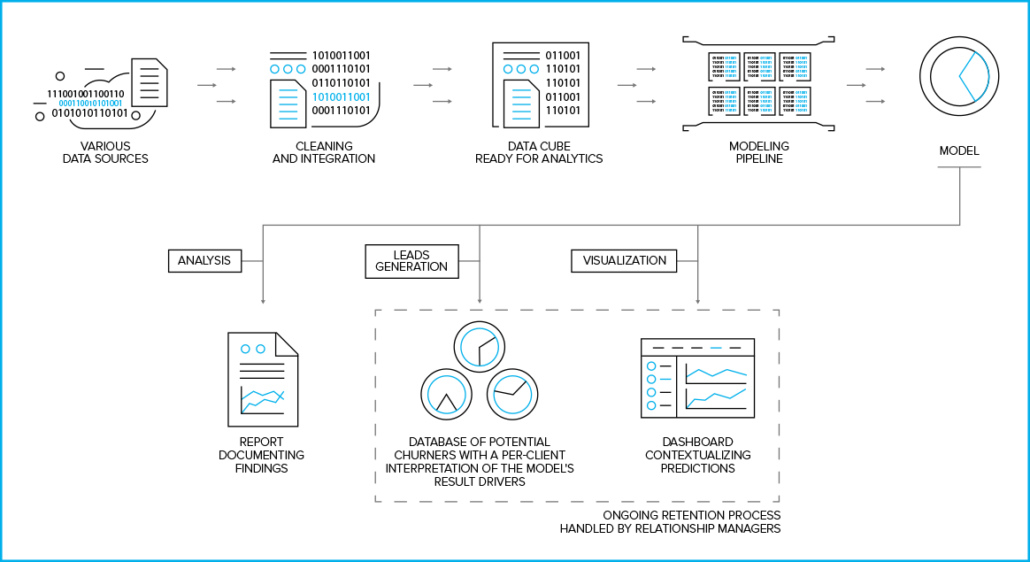
\includegraphics[scale=0.2]{churn}
	\caption{Churn Prediction Analysis.}
\end{figure}

%\section{Result}

%\section{Discussion}

%	\section{Conclusion}
%	The conclusion goes here.
	
	
	
	
	
	% if have a single appendix:
	%\appendix[Proof of the Zonklar Equations]
	% or
	%\appendix  % for no appendix heading
	% do not use \section anymore after \appendix, only \section*
	% is possibly needed
	
	% use appendices with more than one appendix
	% then use \section to start each appendix
	% you must declare a \section before using any
	% \subsection or using \label (\appendices by itself
	% starts a section numbered zero.)
	%
	
	
%	\appendices
%	\section{Proof of the First Zonklar Equation}
%	Appendix one text goes here.
	
	% you can choose not to have a title for an appendix
	% if you want by leaving the argument blank
%	\section{}
%	Appendix two text goes here.
	
	
	% use section* for acknowledgment
	\section*{Acknowledgement}
	The completion of this study could not have been possible without the expertise of Dr Chaw Jun Kit, our beloved supervisor and Professor Lim Tong Ming for encouragement and guiding us during the entire project development.
	
	A debt of gratitude is also owed to the company that provide the customer transaction dataset for us to process in this project.
	
	Next, we also appreciate TAR University College that giving us support in lab facilities to conduct our project and transportation to participate the training provided by dreamcatcher.
	
	Last but not the least, we are grateful to have each other as team mates and always having discussion and meetings for problems solving and work contribution. Thanks to the team cooperation,we had successfully developed the project.
	\newpage
	% Can use something like this to put references on a page
	% by themselves when using endfloat and the captionsoff option.
	\ifCLASSOPTIONcaptionsoff
	\newpage
	\fi
	
	
	
	% trigger a \newpage just before the given reference
	% number - used to balance the columns on the last page
	% adjust value as needed - may need to be readjusted if
	% the document is modified later
	%\IEEEtriggeratref{10}
	% The "triggered" command can be changed if desired:
	%\IEEEtriggercmd{\enlargethispage{-5in}}
	
	% references section
	
	% can use a bibliography generated by BibTeX as a .bbl file
	% BibTeX documentation can be easily obtained at:
	% http://mirror.ctan.org/biblio/bibtex/contrib/doc/
	% The IEEEtran BibTeX style support page is at:
	% http://www.michaelshell.org/tex/ieeetran/bibtex/
	\bibliographystyle{IEEEtran}
	% argument is your BibTeX string definitions and bibliography database(s)
	\bibliography{reference}
	%
	% <OR> manually copy in the resultant .bbl file
	% set second argument of \begin to the number of references
	% (used to reserve space for the reference number labels box)
	
	
	% biography section
	% 
	% If you have an EPS/PDF photo (graphicx package needed) extra braces are
	% needed around the contents of the optional argument to biography to prevent
	% the LaTeX parser from getting confused when it sees the complicated
	% \includegraphics command within an optional argument. (You could create
	% your own custom macro containing the \includegraphics command to make things
	% simpler here.)
	%\begin{IEEEbiography}[{\includegraphics[width=1in,height=1.25in,clip,keepaspectratio]{mshell}}]{Michael Shell}
	% or if you just want to reserve a space for a photo:
	
%	\begin{IEEEbiography}{Michael Shell}
%		Biography text here.
%	\end{IEEEbiography}
%	
%	% if you will not have a photo at all:
%	\begin{IEEEbiographynophoto}{John Doe}
%		Biography text here.
%	\end{IEEEbiographynophoto}
%	
%	% insert where needed to balance the two columns on the last page with
%	% biographies
%	%\newpage
%	
%	\begin{IEEEbiographynophoto}{Jane Doe}
%		Biography text here.
%	\end{IEEEbiographynophoto}
	
	% You can push biographies down or up by placing
	% a \vfill before or after them. The appropriate
	% use of \vfill depends on what kind of text is
	% on the last page and whether or not the columns
	% are being equalized.
	
	%\vfill
	
	% Can be used to pull up biographies so that the bottom of the last one
	% is flush with the other column.
	%\enlargethispage{-5in}
	
	
	
	% that's all folks
\end{document}